\chapter{Results}
\label{results}
This chapter presents the results achieved during the first part of this project. In a first part, we introduce the tools we use (libraries, datasets). A second part describes our methodology and results regarding the reproduction of state of the art.

\section{Methodology}
As explained in Section \ref{sota}, state of the art \acrshort{lic} models provide great results: they provide encoding of images that contain very few bits while preserving the images quality. However, these models require a lot of processing power making them unsuitable for realtime application on resource constrained devices. The goal of this project is to explore solutions to reduce the processing power used by these models, leading to realtime image compression/decompression on such devices. In order to do that, it is necessary to have access to the state of the art \acrshort{lic} models, the image datasets used to train them and enough processing power to train such models.

CompressAI \cite{compressai} is a Python library for learned compression. Based on the well known machine learning library PyTorch, compressAI provides custom operations, layers and models for deep learning based data compression and pre-trained end-to-end compression models for \acrshort{lic}. Amongs the pre-trained models is the model from Ballé et al.\cite{ballemshj18} that will be used throughout the project.

Usually, researchers train their models on the OpenImages dataset \cite{openimages} but pre-trained models on compressAI have been trained on the Vimeo90K dataset \cite{xue2019video}. In order to perform proper model comparisons, the Vimeo dataset will be used for training in this project. For testing, two datasets will be used: the Kodak dataset \cite{kodak} and the dataset from the \acrfull{clic} \cite{clic}.

The computing power required for training and using models will be provided by the GPU cluster of Télécom Paris.

\section{Results Reproduction}
In a research project, reproducing state of the art results is key. The first thing to do is to ensure that our work environnement is correct by reproducing results from articles. This also provides a shared baseline results between papers and our work, that can be used to compare our future results.

As experiments parameters are not disclosed in the papers we studied, we try to reproduce results from the compressAI library, taht is to say: achieve the same results as the pre-trained models from the model zoo.

The training methodology used by compressAI is described in the documentation \cite{compressai_train}. Models were trained between 4 and 5 million steps on 256x256 image patches randomly extracted and cropped from the Vimeo90K dataset. The batch size is 16 or 32 (we choose 16). The initial learning rate is 1e-4 and decreases over time (it is divided by 2 when the evaluation loss reaches a plateau). Two different metrics can be used: MSE or MS-SSIM. We keep the default metric (MSE) which corresponds to using the following loss function: \(L = \lambda * 255^{2} * D + R\) with \(D\) and \(R\) respectively the mean distortion and the mean estimated bit-rate. The parameter \(\lambda\) allows to adjust the tradeoff between compression and image quality. Higher values give more importance to distortion encouraging the model to produce reconstructed images with high quality at the expense of bit-rate. Inversely, lower values of \(\lambda\) imply more compression and more data loss. CompressAI proposes 8 pre-trained models with different values of \(\lambda\) represented by the argument \textsf{quality}. The correspondance between this argument and the value of \(\lambda\) is summarised in Table \ref{tab}. It is important to note that the \textsf{quality} argument in compressAI also impacts the network architecture.

\begin{table}[]
    \centering
    \begin{tabular}{|l|c|c|c|c|c|c|c|c|}
    \hline
    \textsf{quality}                      & 1 & 2 & 3 & 4 & 5 & 6 & 7 & 8 \\ \hline
    Value of \(\lambda\) for MSE & 0.0018 & 0.0035 & 0.0067 & 0.0130 & 0.0250 & 0.0483 & 0.0932 & 0.1800 \\ \hline
    \end{tabular}
    \caption{Correspondance between the argument \textsf{quality} in compressAI and the value of \(\lambda\) when using MSE}
    \label{tab}
\end{table}

This part of the project is divided in two parts. First, we try to train a single model and compare it to other pre-trained models. Then we train several models in order to produce rate-distortion curves.

\subsection{Single Model}
Using the training script provided by compressAI and following the same methodology, we train a model for \(5 \times 24\) hours (approximately 700 epochs). Eventhough weights are loaded from previous checkpoint at the beginning of each training, this is different than training the model for 6 hours straight due to the change of learning rate over time (for each training session the learning rate is set back to 1e-4). We use the default value for \(\lambda\) (1e-2) and the architecture corresponds to setting the compressAI argument \textsf{quality} to 3.

After training we can evaluate our model. First, we try a single inference with this newly trained model. Figure \ref{balle_repro_1} shows that the reconstructed image (middle) is visually close to the original image. However, the difference between the two images (right) reveals that there are a lot of differences. These differences are compared in the part of the image that contains details. These parts are often refered as containing high frequencies an are particularly hard to compress as opposed to low frequency areas (like the sky in this picture) that do not contain a lot of information and are easier to compress.

\begin{figure}
    \centering
    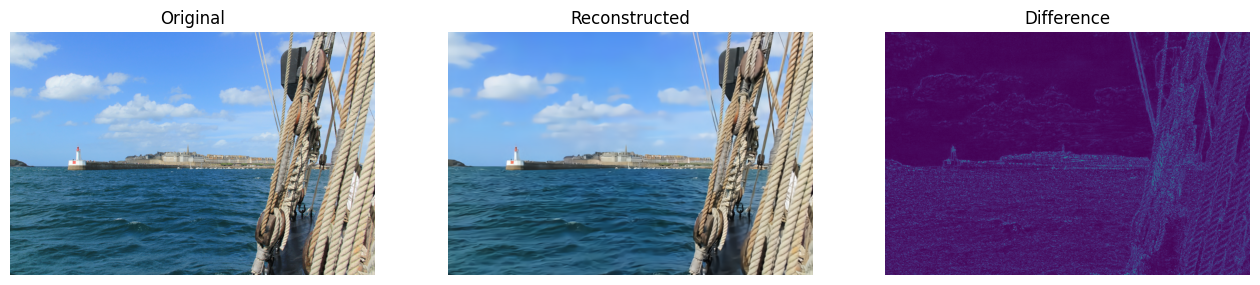
\includegraphics[width=15cm]{img/balle_repro_1.png}
    \caption{Comparison of the reconstrcuted with the original image}
    \label{balle_repro_1}
\end{figure}

Figure \ref{balle_repro_2} shows encoding of the image at the same bit-rate using different methods. It is clear that the network is the more accurate among the three methods used: the reconstructed image is closer to the original image. JPEG introduces a lot of artifacts (blocs) and Webp does not retains as much details as the network, especially in the water.

\begin{figure}
    \centering
    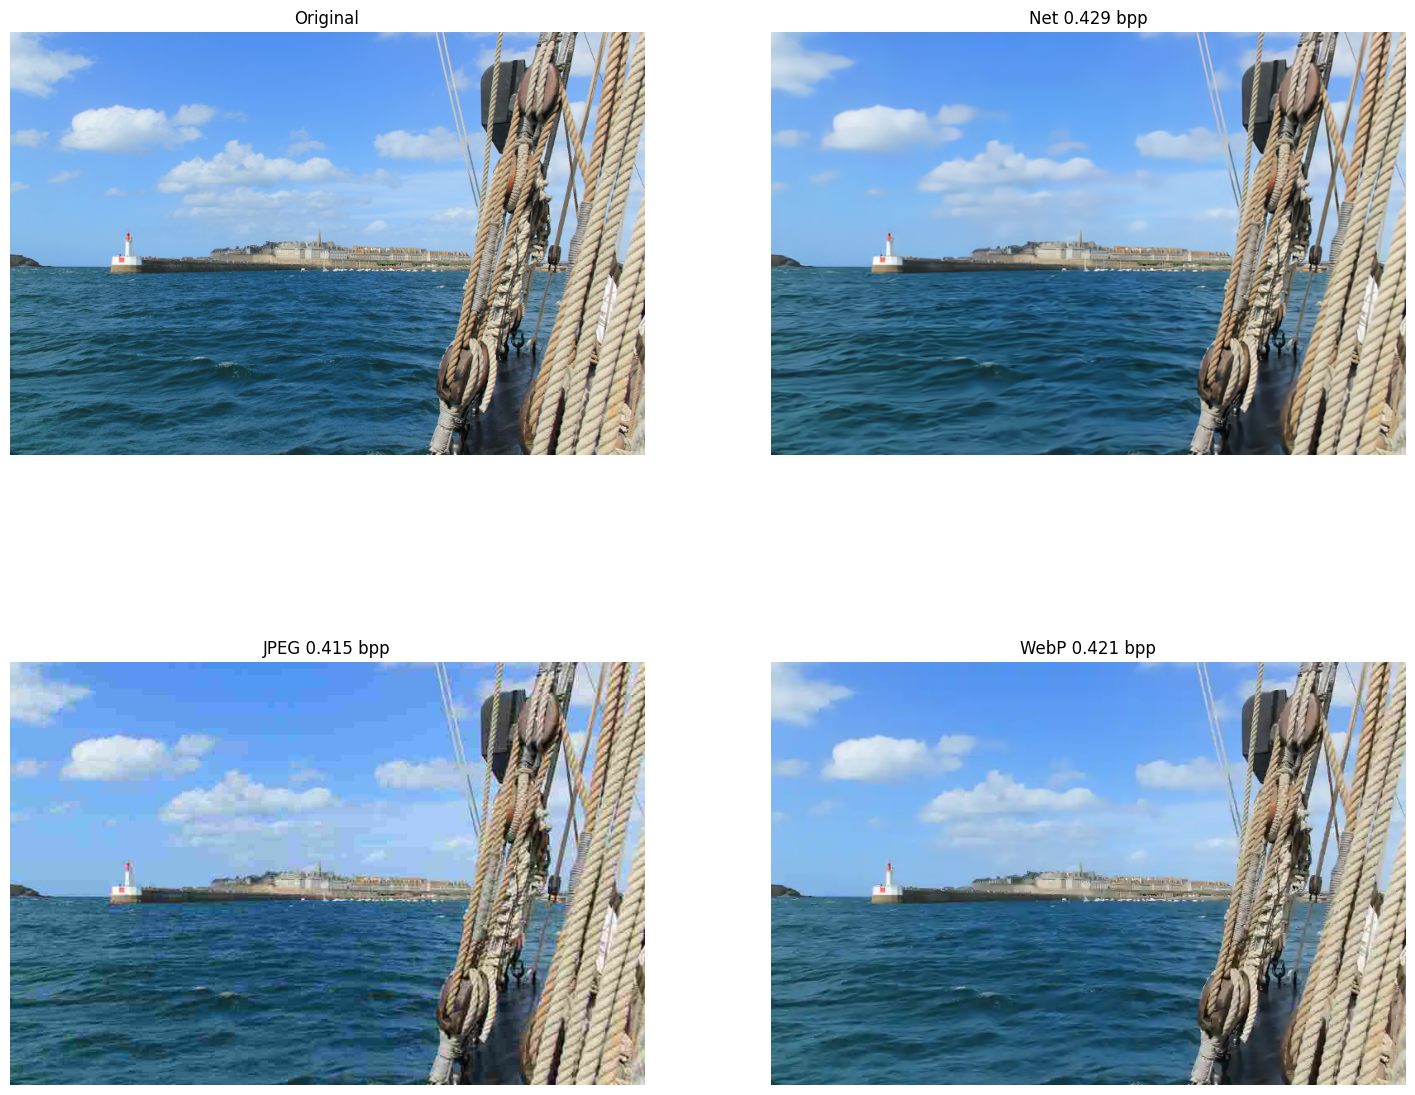
\includegraphics[width=15cm]{img/balle_repro_2.png}
    \caption{Comparison to classical codecs: quality coparison at similar bit-rate}
    \label{balle_repro_2}
\end{figure}

For the same distortion rate, our model manages has the smallest bit-rate out of the three methods, that is to say: for the same visual quality, measured by the \acrful{psnr}, the image is more compressed. Figure \ref{balle_repro_3} shows that it achieves less than 0.5 bits per pixel whereas traditional compression methods like Webp or JPEG achieve respectively 0.698 and 1.054 bit per pixels.

\begin{figure}
    \centering
    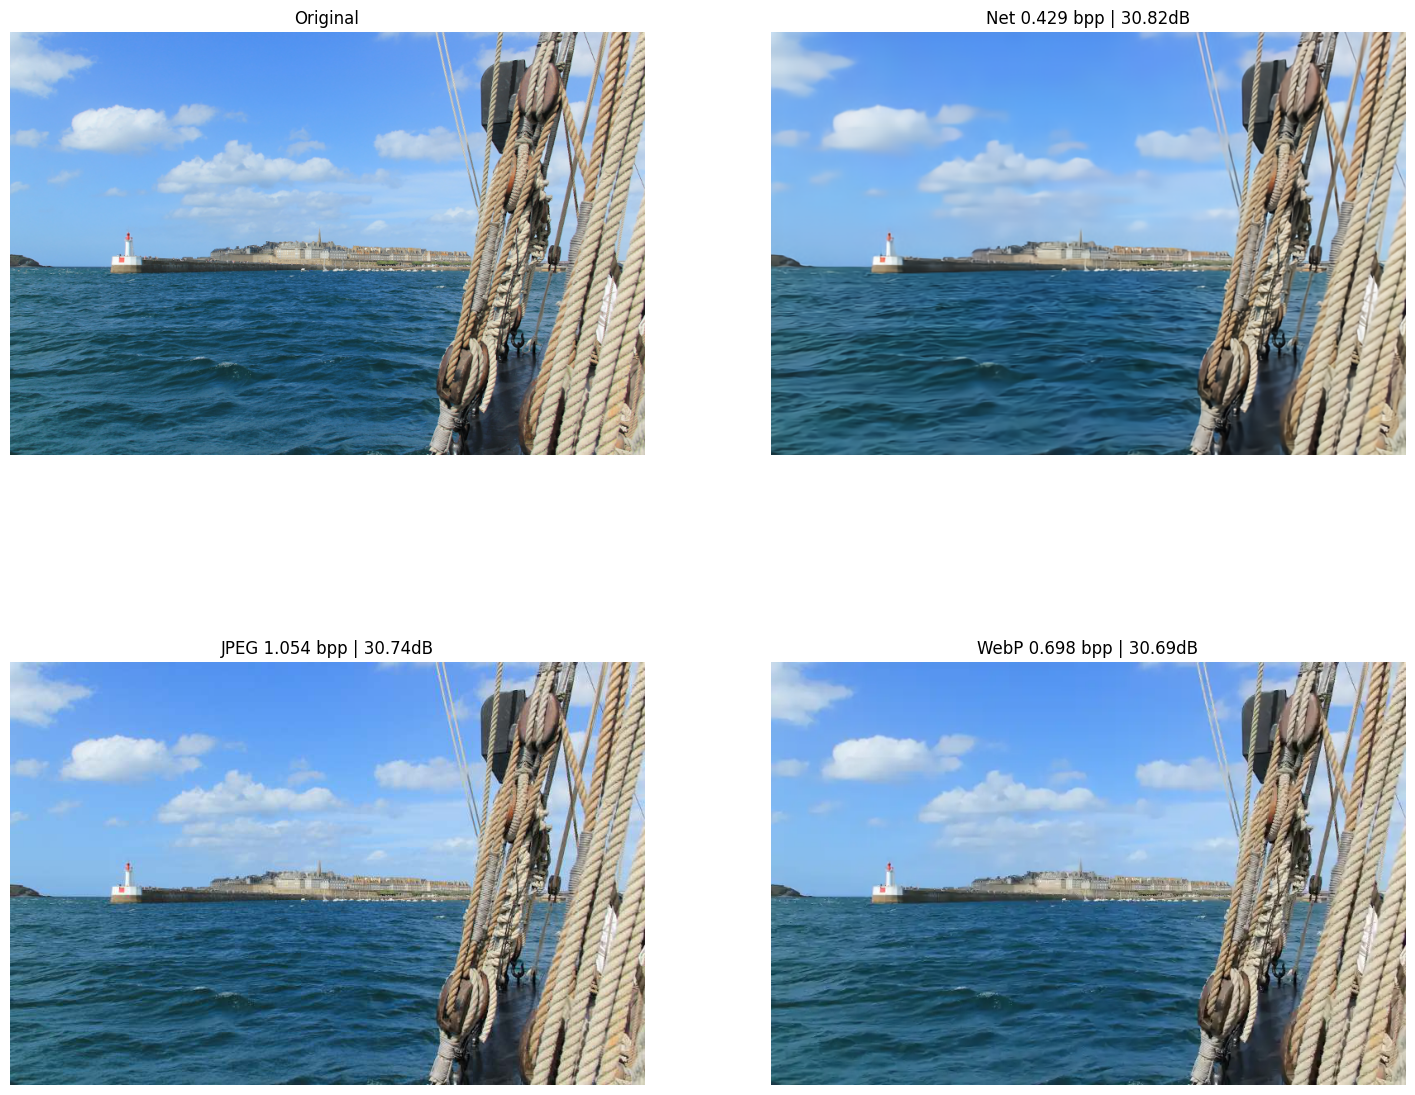
\includegraphics[width=15cm]{img/balle_repro_3.png}
    \caption{Comparison to classical codecs: bit-rate coparison at similar PSNR}
    \label{balle_repro_3}
\end{figure}

Similar results are observed on Figure \ref{balle_repro_4} which is based on MS-SSIM, another method to measure visual fidelity.

\begin{figure}
    \centering
    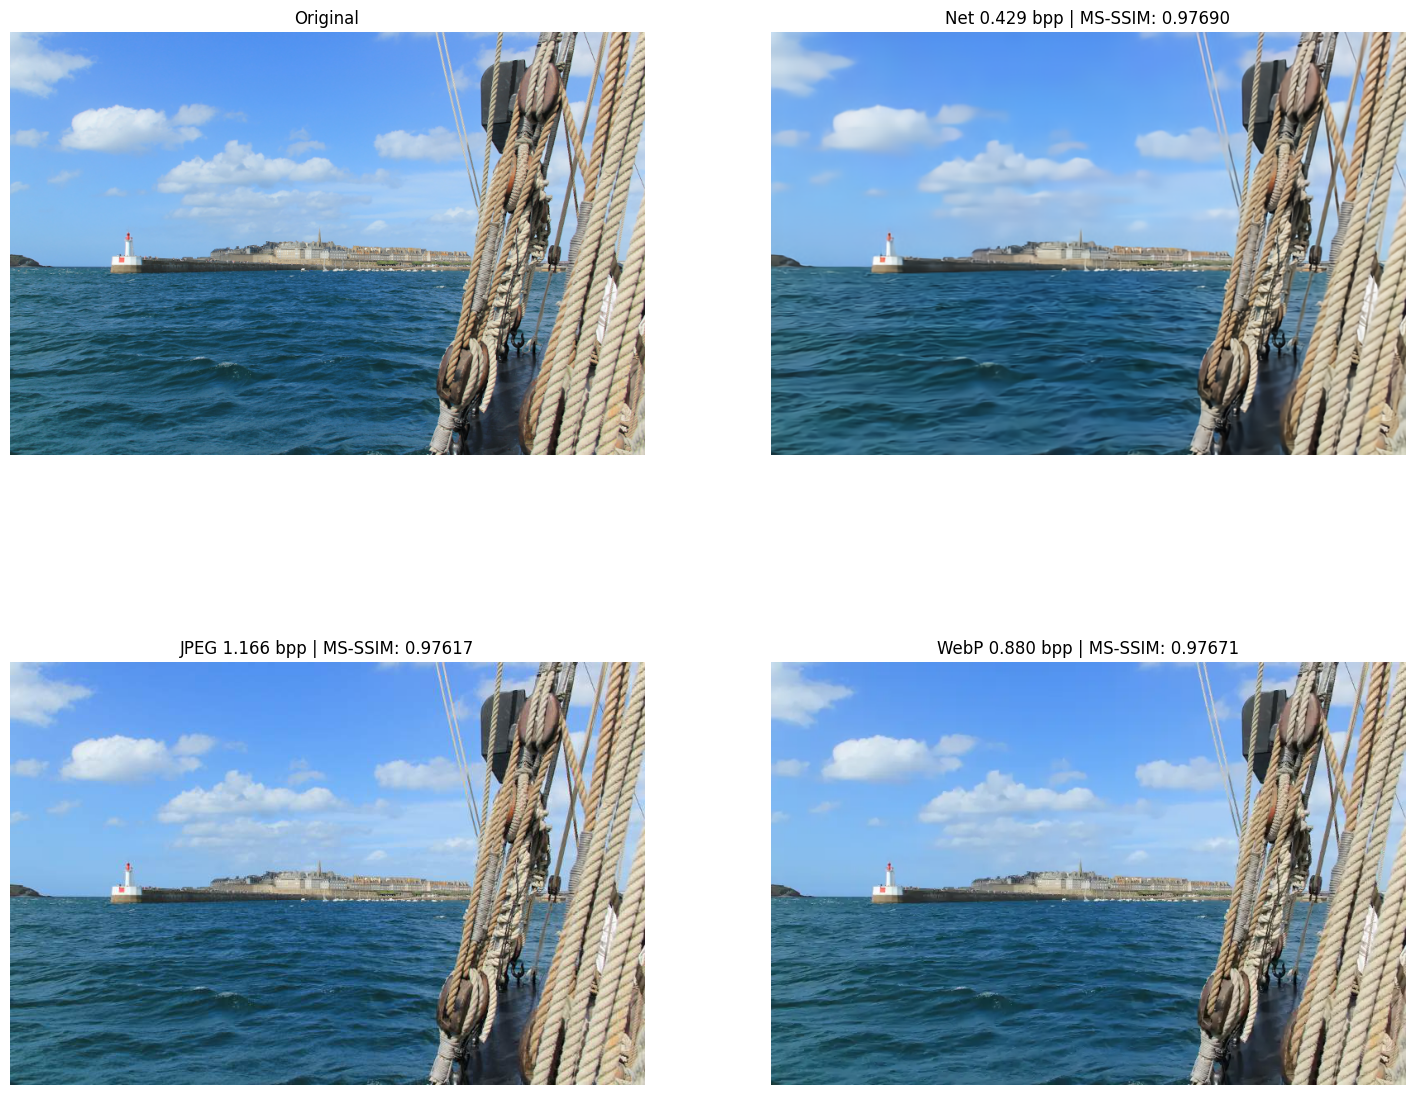
\includegraphics[width=15cm]{img/balle_repro_4.png}
    \caption{Comparison to classical codecs: bit-rate coparison at similar MS-SSIM}
    \label{balle_repro_4}
\end{figure}

Finally, we compare our models to other \acrshort{lic} models accessbible in the compressAI model zoo. Figure \ref{balle_repro_5} allows to compare visual results from our model at three stages of the training and various pre-trained models. Results are visually close but, by zooming, it is clear that our models retain more details than the other pre-trained models (for intance in the ropes). This is coherent with Figure \ref{balle_repro_6} that shows that our models are more focused on quality at the expense of bit-rate (located in the top right of the plot). Other models perform worse in term of image quality but achieve a lower compression rate (bottom left of the plot).

\begin{figure}
    \centering
    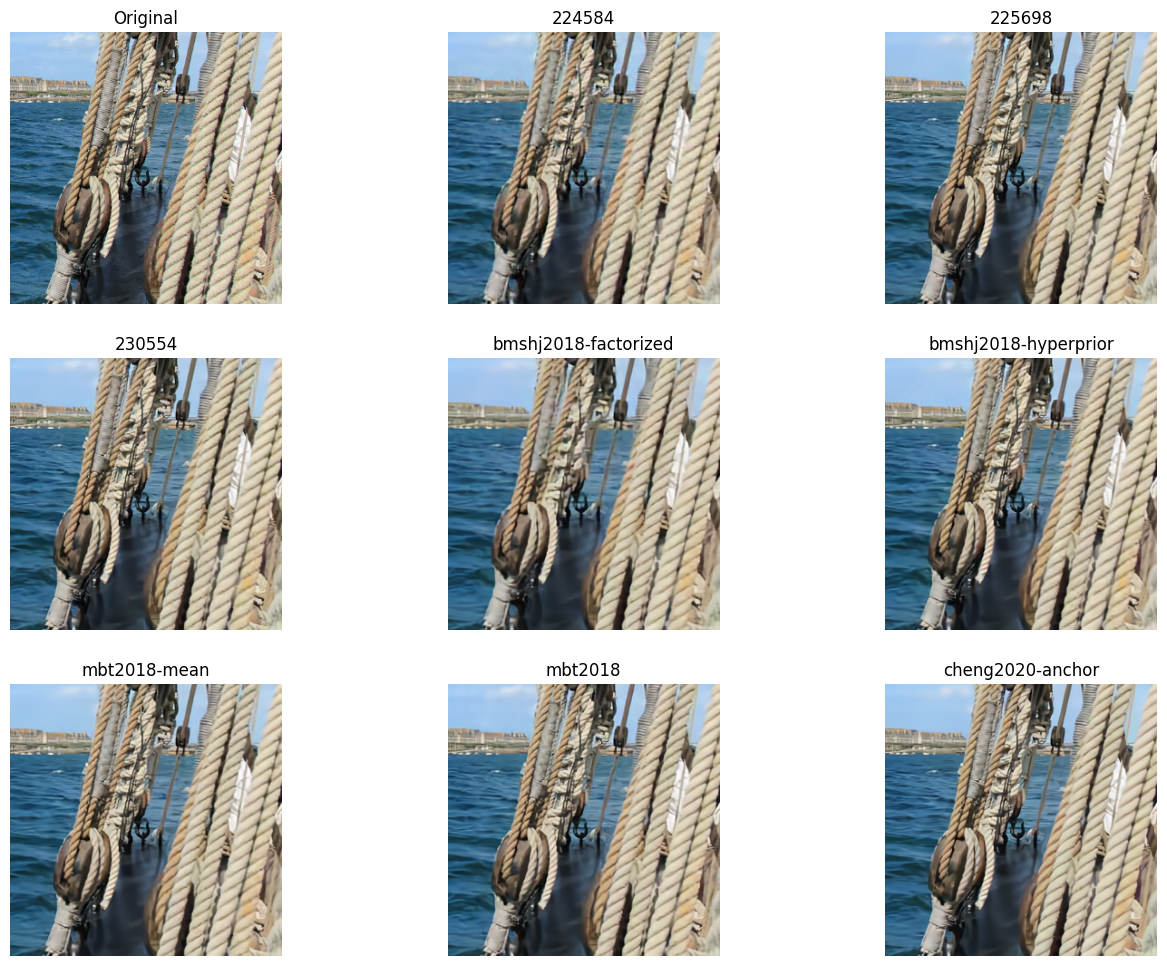
\includegraphics[width=15cm]{img/balle_repro_5.png}
    \caption{Comparison to other \acrshort{lic} models: image reconstruction}
    \label{balle_repro_5}
\end{figure}

\begin{figure}
    \centering
    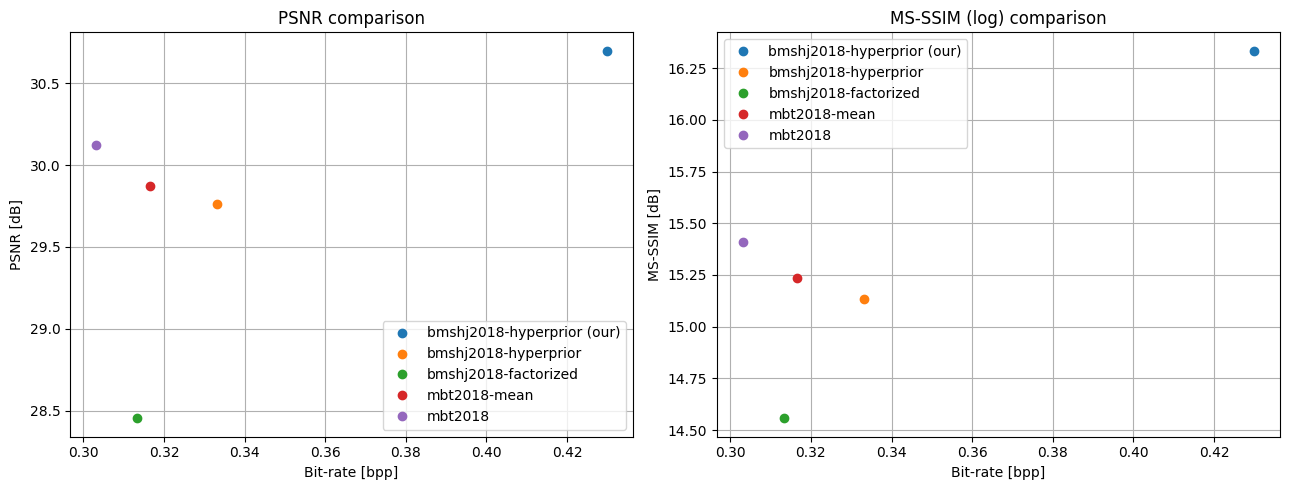
\includegraphics[width=15cm]{img/balle_repro_6.png}
    \caption{Comparison to other \acrshort{lic} models: rate-distortion curves}
    \label{balle_repro_6}
\end{figure}

This section show that we are able to train a \acrshort{lic} model that can compress and reconstruct images while mostly preserving its content. Our models perform better than deterministic codecs like JPEG or Webp but our models does not produce the same results as the pre-trained ones. It should be noted that, at this point, we are mainly checking if training is working properly on the GPU cluster and that we are now comparing models that were trained differently. Next section focuses more on the models parameters and the impact on the bit-rate/distortion tradeoff.

\subsection{Rate-Distortion Curves}
Using the training script provided by compressAI and following the same methodology, we train 8 different models: one for each value of \textsf{quality}. That is to say, one for each couple of \(\lambda\) value and corresponding model architecture. However, to quickly achieve comparable results, we limit the number of epochs to 65, just under what the GPU cluster is able to compute in 24 hours.

This method allows us to compare models more precisely by taking into account the bit-rate/distortion tradeoff induced by the value of \(\lambda\) parameter. Figure \ref{bdpsnr_1} and \ref{bdpsnr_2} show image reconstruction results from our models and pre-trained models for each value of \(\lambda\). There is a clear change in image quality between images in the top-left corresponding to lower values of \(\lambda\) (low bit-rate and low quality) and images in the bottom-right corner correponding to higher values of \(\lambda\) (high bit-rate and high quality) for both our models and pre-trained models.

\begin{figure}[H]
    \centering
    \subfloat[Our networks]{{\includegraphics[width=8.5cm]{/home/fabien/TSP/3A/PRIM/bdpsnr/test_res/20241129_085637/networks_kodak_kodim14.png} \label{bdpsnr_1:a}}}
    \subfloat[Pre-trained networks]{{\includegraphics[width=8.5cm]{/home/fabien/TSP/3A/PRIM/bdpsnr/test_res/20241129_085637/pretrained_networks_kodak_kodim14.png} \label{bdpsnr_1:b}}}
    \caption{Reconstruction results on image 14 of the Kodak dataset}
    \label{bdpsnr_1}
\end{figure}

\begin{figure}[H]
    \centering
    \subfloat[Our networks]{{\includegraphics[width=8.5cm]{/home/fabien/TSP/3A/PRIM/bdpsnr/test_res/20241129_085637/networks_kodak_kodim15.png} \label{bdpsnr_2:a}}}
    \subfloat[Pre-trained networks]{{\includegraphics[width=8.5cm]{/home/fabien/TSP/3A/PRIM/bdpsnr/test_res/20241129_085637/pretrained_networks_kodak_kodim15.png} \label{bdpsnr_2:b}}}
    \caption{Reconstruction results on image 15 of the Kodak dataset}
    \label{bdpsnr_2}
\end{figure}

We are also able to produce rate-distortion curves for each image of the testing dataset in order to compare our models with pre-trained models. Figure \ref{bdpsnr_3} show an example of one of this curve. This shows that for lower bit-rate (lower values of \(\lambda\)) our model is very similar to the pre-trained models but there is a slight difference for higher bit-rates where our models do not reach the same level of image quality.

\begin{figure}
    \centering
    \includegraphics[width=15cm]{/home/fabien/TSP/3A/PRIM/bdpsnr/test_res/20241129_085637/curve_kodak_kodim15.png}
    \caption{Rate-distortion curve for image 14 of the Kodak dataset}
    \label{bdpsnr_3}
\end{figure}

By averaging metrics on the test dataset, we create an average rate-distortion curve for the entire test dataset. This curve is shown in Figure \ref{bdpsnr_4}. Results are similar to those obtained in Figure \ref{bdpsnr_3}: our models are very close to pre-trained models with a little disadvantage when dealing with higher bit-rates.

\begin{figure}
    \centering
    \includegraphics[width=15cm]{/home/fabien/TSP/3A/PRIM/bdpsnr/test_res/20241129_085637/avg_curve_kodak.png}
    \caption{Average rate-distortion curve for the Kodak dataset}
    \label{bdpsnr_4}
\end{figure}

These results show that we are able to reproduce state of the art results for \acrshort{lic} using publicly available datasets and the processing power of the Télécom Paris GPU cluster.

\section{Future Work}
Current results prove that we are able to achieve close to, if not state of the art \acrshort{lic} results on traditional hardware. Future work will focus on improving models to work on power constrained platforms (like FPGA) by using techniques like pruning, quantisation and knowledge distillation. We will start by implementing and evaluating these techniques to work on single images whereupon we will add the realtime constraint.